\chapter{На каких языках программирования пишутся операционные системы}
\label{ch:operating-sysmets}

В статье исследуется объект Викиданных <<операционная система>> (operating system) и его свойства. В каждом из разделов представлены задачи, решённые с помощью SPARQL-запросов. В их числе: нахождение экземпляров объекта <<операционная система>>, построение списка операционных систем (ОС) по предку, по времени создания, по языку, на котором написана ОС. Также построена гистограмма, показывающая количество программ, написанных на том или ином языке программирования, и долю того, сколько из них работает под той или иной ОС. У многого программного обеспечения не указан язык программирования, на котором оно разрабатывалось. Для улучшения результатов решения вышеописанных задач отдельные объекты Викиданных были дополнены свойством <<язык программирования>>.

\section{Полнота данных}
По данным на 2017 год с сайта www.operating-system.org удалось установить что существует порядка 611 операционных систем (не учитывая дистрибутивы Linux'а, коих количество превышает количество самих операционных систем). В то время как викиданные содержат информацию лишь о 510 операционных системах. И если просмотреть достаточно большое количество объектов из запрос, то станет ясно еще и то, что много из них еще и не очень хорошо заполнены, а то и вовсе практически пусты.

В 2020 году викиданные содержат информацию о 1086 операционных системах, что свидетельствует о значительных изменениях, однако большое количество объектов по-прежнему плохо заполнены. Из этого можно сделать вывод о неполноте викиданных.

\section{Языки программирования, используемые для написания операционных система}
Если взглянуть на количество операционных систем, для которых указано свойство <<язык программирования>>, то можно увидеть что из 1086 объектов это свойство заполнено лишь у 116. Но по существующим данным на рис.~\ref{fig:count-os-written-on-languages} можно определить, что большинство операционных систем написаны на языке программирования C. 
\begin{figure*}[h!]
	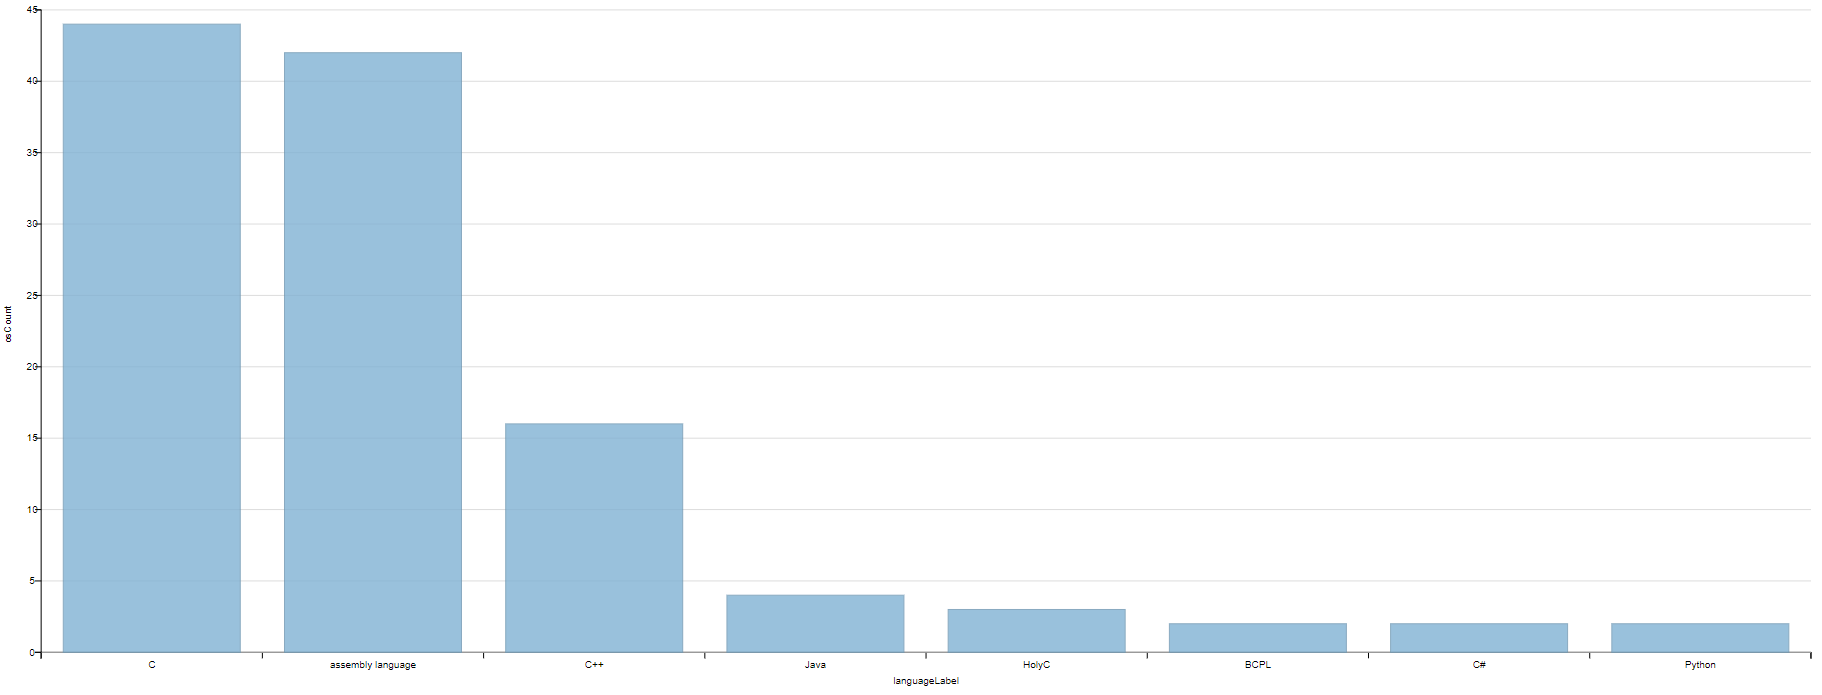
\includegraphics{./chapter/operating_system/count-os-written-on-languages.png}
	\caption{Количество операционных систем, написанных на языках программирования (данные на 2020 год.)}
	\label{fig:count-os-written-on-languages}
\end{figure*}

Такие данные вызывают большие сомнения.